% Options for packages loaded elsewhere
\PassOptionsToPackage{unicode}{hyperref}
\PassOptionsToPackage{hyphens}{url}
%
\documentclass[
]{article}
\usepackage{amsmath,amssymb}
\usepackage{lmodern}
\usepackage{iftex}
\ifPDFTeX
  \usepackage[T1]{fontenc}
  \usepackage[utf8]{inputenc}
  \usepackage{textcomp} % provide euro and other symbols
\else % if luatex or xetex
  \usepackage{unicode-math}
  \defaultfontfeatures{Scale=MatchLowercase}
  \defaultfontfeatures[\rmfamily]{Ligatures=TeX,Scale=1}
\fi
% Use upquote if available, for straight quotes in verbatim environments
\IfFileExists{upquote.sty}{\usepackage{upquote}}{}
\IfFileExists{microtype.sty}{% use microtype if available
  \usepackage[]{microtype}
  \UseMicrotypeSet[protrusion]{basicmath} % disable protrusion for tt fonts
}{}
\makeatletter
\@ifundefined{KOMAClassName}{% if non-KOMA class
  \IfFileExists{parskip.sty}{%
    \usepackage{parskip}
  }{% else
    \setlength{\parindent}{0pt}
    \setlength{\parskip}{6pt plus 2pt minus 1pt}}
}{% if KOMA class
  \KOMAoptions{parskip=half}}
\makeatother
\usepackage{xcolor}
\IfFileExists{xurl.sty}{\usepackage{xurl}}{} % add URL line breaks if available
\IfFileExists{bookmark.sty}{\usepackage{bookmark}}{\usepackage{hyperref}}
\hypersetup{
  pdfauthor={Daniel Correia},
  hidelinks,
  pdfcreator={LaTeX via pandoc}}
\urlstyle{same} % disable monospaced font for URLs
\usepackage{graphicx}
\makeatletter
\def\maxwidth{\ifdim\Gin@nat@width>\linewidth\linewidth\else\Gin@nat@width\fi}
\def\maxheight{\ifdim\Gin@nat@height>\textheight\textheight\else\Gin@nat@height\fi}
\makeatother
% Scale images if necessary, so that they will not overflow the page
% margins by default, and it is still possible to overwrite the defaults
% using explicit options in \includegraphics[width, height, ...]{}
\setkeys{Gin}{width=\maxwidth,height=\maxheight,keepaspectratio}
% Set default figure placement to htbp
\makeatletter
\def\fps@figure{htbp}
\makeatother
\setlength{\emergencystretch}{3em} % prevent overfull lines
\providecommand{\tightlist}{%
  \setlength{\itemsep}{0pt}\setlength{\parskip}{0pt}}
\setcounter{secnumdepth}{-\maxdimen} % remove section numbering
\newlength{\cslhangindent}
\setlength{\cslhangindent}{1.5em}
\newlength{\csllabelwidth}
\setlength{\csllabelwidth}{3em}
\newlength{\cslentryspacingunit} % times entry-spacing
\setlength{\cslentryspacingunit}{\parskip}
\newenvironment{CSLReferences}[2] % #1 hanging-ident, #2 entry spacing
 {% don't indent paragraphs
  \setlength{\parindent}{0pt}
  % turn on hanging indent if param 1 is 1
  \ifodd #1
  \let\oldpar\par
  \def\par{\hangindent=\cslhangindent\oldpar}
  \fi
  % set entry spacing
  \setlength{\parskip}{#2\cslentryspacingunit}
 }%
 {}
\usepackage{calc}
\newcommand{\CSLBlock}[1]{#1\hfill\break}
\newcommand{\CSLLeftMargin}[1]{\parbox[t]{\csllabelwidth}{#1}}
\newcommand{\CSLRightInline}[1]{\parbox[t]{\linewidth - \csllabelwidth}{#1}\break}
\newcommand{\CSLIndent}[1]{\hspace{\cslhangindent}#1}
\ifLuaTeX
  \usepackage{selnolig}  % disable illegal ligatures
\fi
\thispagestyle{empty}
\author{Daniel Correia}
\date{}

\begin{document}

\hypertarget{a-few-notes-on-deconvolution-of-xafs-spectra}{%
\section{A few notes on deconvolution of XAFS
spectra}\label{a-few-notes-on-deconvolution-of-xafs-spectra}}

\begin{center}
Daniel Correia
\end{center}

\begin{quote}
An ostensibly more noise-tolerant deconvolution algorithm is (poorly)
implemented in Larch; results are not clearly superior. Real-world
results from the VLS-PGM are re-processed and yield useable fidelity. An
interface to the existing inverse filtering deconvolution is added to
demeter/Athena. Non-stationary kernels are discussed.
\end{quote}

\begin{center}
	\makebox[\textwidth]{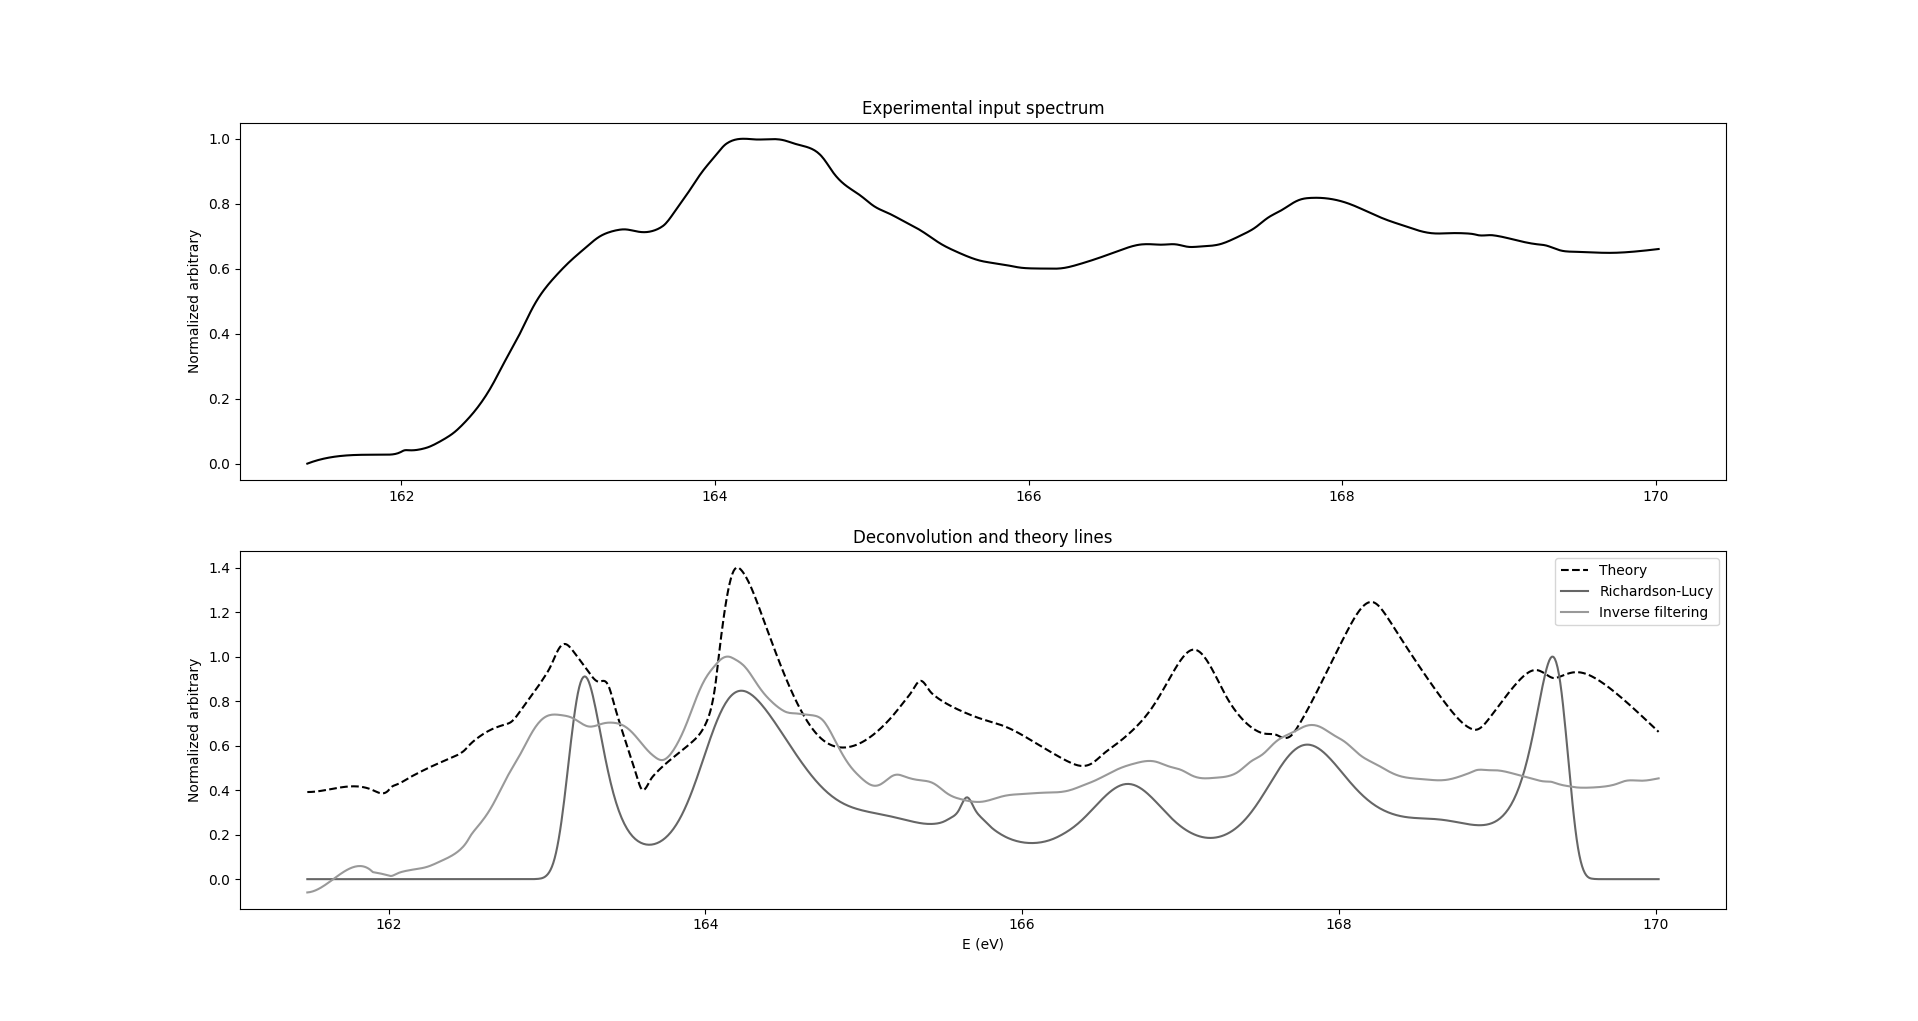
\includegraphics[width=\paperwidth]{Zn_Cu_output.png}}
\end{center}

Pratt et al. (\protect\hyperlink{ref-Highresolution2007}{2007}) perform
XANES on a variety of ZnS sphalerite samples and compare FLY to a nifty
ab initio model. They find limited correspondence between theory and
experiment unless the predicted spectra are filtered and broadened by 1
eV, accounting for all the sources of line uncertainty in the
experiment, in which case a perfect fit is found.

In this figure, two deconvolution algorithms (bottom, solid) are used to
pare off a gaussian with \(\pm\sigma=0.5 \text{ eV}\) from the same
experimental data (top), the reverse procedure to that used in Pratt et
al.

\pagebreak

Very surprisingly, the small inflection point near 166 eV (what is this
feature?) predicted by theory is accurately reconstructed by the L-R
algorithm, even though no corresponding feature is obviously present in
the input data. On the other hand, a poor showing is consistenly seen in
the ripple near 170 eV.

A relatively wide slit width of 100 um was used for this experiment,
which may have contributed to the success of deconvolution.

\hypertarget{introduction}{%
\subsubsection{Introduction}\label{introduction}}

\emph{(note: this was written by someone with perhaps an hour's
experience in XAS, as a learning experience; all statements are almost
certainly false.)}

Notes and code from this paper are available at
https://github.com/0xDBFB7/synchrotron-project; Forks of larch
(\protect\hyperlink{ref-Larch2013}{Newville 2013}) and
demeter(\protect\hyperlink{ref-ATHENA2005}{Ravel and Newville 2005})
used are https://github.com/0xDBFB7/xraylarch and
https://github.com/0xDBFB7/demeter.

In papers characterizing the VLS-PGM{[}Zuin, Hu, and Sham
(\protect\hyperlink{ref-zuin2007early}{2007}){]}(\protect\hyperlink{ref-VLSPGM2007a}{Hu
et al. 2007}) and similar beamlines, the resolving power
\(\lambda/\text{d}\lambda = E/\text{d}E\) of the system is often a key
point of comparison. However, this resolving power does not perhaps seem
to represent an ultimate ``information-theoretic'' limit, but rather
seems to mostly reflect the fineness of the output spectrum of the
monochromator (see, \protect\hyperlink{ref-XRay1991}{Agarwal 1991, chap.
9.5}, ``Plane crystal spectrograph'').

Purely for amusement, the question arose of what ultimate resolution
could be achieved if the effect of the monochromator spectrum was
corrected for.

With modern detectors and techniques, I assume that circumstances where
deconvolution is part of a good experimental design are probably rather
rare. Nehzati et al. (\protect\hyperlink{ref-High2021}{2021}), for
instance, discuss a HERFD-XAS technique that can natively probe at
sub-linewidth resolutions. It seems better to use an inherently
higher-resolution technique then to try to extract ambiguous peaks from
mud. The L-R algorithm has several knobs that can be turned to suit
different hypotheses (\protect\hyperlink{ref-Retraction2018}{Bergmann et
al. 2018}); if careful attention is not taken in following the strict
validation procedures listed
(\protect\hyperlink{ref-Deconvolving2007}{Fister et al. 2007}) (as was
neglected here) many conclusions could be argued for using the same
data.

An X-ray spectrum observed from experiment represents the convolution of
many different sources of broadening. Excellent discussion can be found
in (\protect\hyperlink{ref-XRay1991}{Agarwal 1991}), particularly
chapters 4.4, 4.5.3 and 4.7, and the larch manual page
(\protect\hyperlink{ref-13a}{{``13.2. {XAFS}: {Pre-edge Subtraction},
{Normalization}, and Data Treatment --- Xraylarch 0.9.57
Documentation''} n.d.}) on deconvolution. Sources of experimental error
are listed by Outka and Stöhr (\protect\hyperlink{ref-Curve1988}{1988}),
and include an \(I\) term for beam intensity, an \(M_i\) term for
monochromator first and higher orders, a \(D\) term for detector
transfer functions, and finally various sample contamination terms
\(S_e\).

The most severe in cases of high medium Z is lifetime broadening, a
consequence of the uncertainty principle. This goes as

\[\Gamma\approx A + RZ^4\]

The next most significant contribution is experimental. There are many
ways of correcting for instruments
(\protect\hyperlink{ref-Curve1988}{Outka and Stöhr 1988}); division by
reference lines, subtraction, etc.

Since the resolving power of the monochromator can be simulated, there
is considerable information available for deconvolution. A very
analogous procedure is performed with some high-performance digitizers
(\protect\hyperlink{ref-Bandwidth1994}{\textbf{Bandwidth1994?}}) in the
time domain rather than the energy domain.

\hypertarget{deconvolution-algorithms}{%
\subsubsection{Deconvolution
algorithms}\label{deconvolution-algorithms}}

Larch has a built-in support for deconvolution using numpy's
`deconvolve', and can deconvolve a gaussian or laplacian kernel. This
performs a very basic fourier-transform Inverse Filtering deconvolution
with a final Golay filtering step. In general, inverse filtering is held
to perform poorly in the presence of noise and imperfect knowledge.

Advanced techniques exist
(\protect\hyperlink{ref-Extraction2000}{Klementiev 2000}); these seemed
daunting for the time allotted.

(\protect\hyperlink{ref-Deconvolving2007}{Fister et al. 2007}) use an
algorithm based on the Lucy-Richardson, an iterative method, with a
gaussian smoothing step to suppress noise. I had not anticipated the
success of IF. This is the L-R algorithm used in the plot above.

One advantage of the L-R method is that it only requires the forward
convolution to exist, which allows a bit more flexibility. The
convergence properties seen in my implementation is not similar to that
by Fister et al, so there are almost certainly lingering bugs.

\hypertarget{non-stationary-kernels}{%
\subsubsection{Non-stationary kernels}\label{non-stationary-kernels}}

One impediement to deconvolving to the maximum resolution, especially in
the case of the VLS-PGM, is the significant non-flatness of the
monochromator's output spectrum across the energy window.

In the worst-case, the resolving power can vary between 27000 to 15000
between 10 and 20 eV.

In practice, segments of spectrum requiring ultra-high-resolution seem
probably unlikely to be very much wider than a few tens of eV, so the
variation in spectrum seems likely to be small.

In signal theory this property is known as a non-stationary or varying
kernel or PSF. An interesting technique using eigen-kernel
decomposition, suitable for deconvolving energy-variant kernels of
arbitrary (non-guassian structure), is listed in
(\protect\hyperlink{ref-Deconvolution2002}{Lauer 2002}).

Another technique - only valid for gaussian kernels - is to stretch and
warp the energy domain to create a uniform broadening, like so:

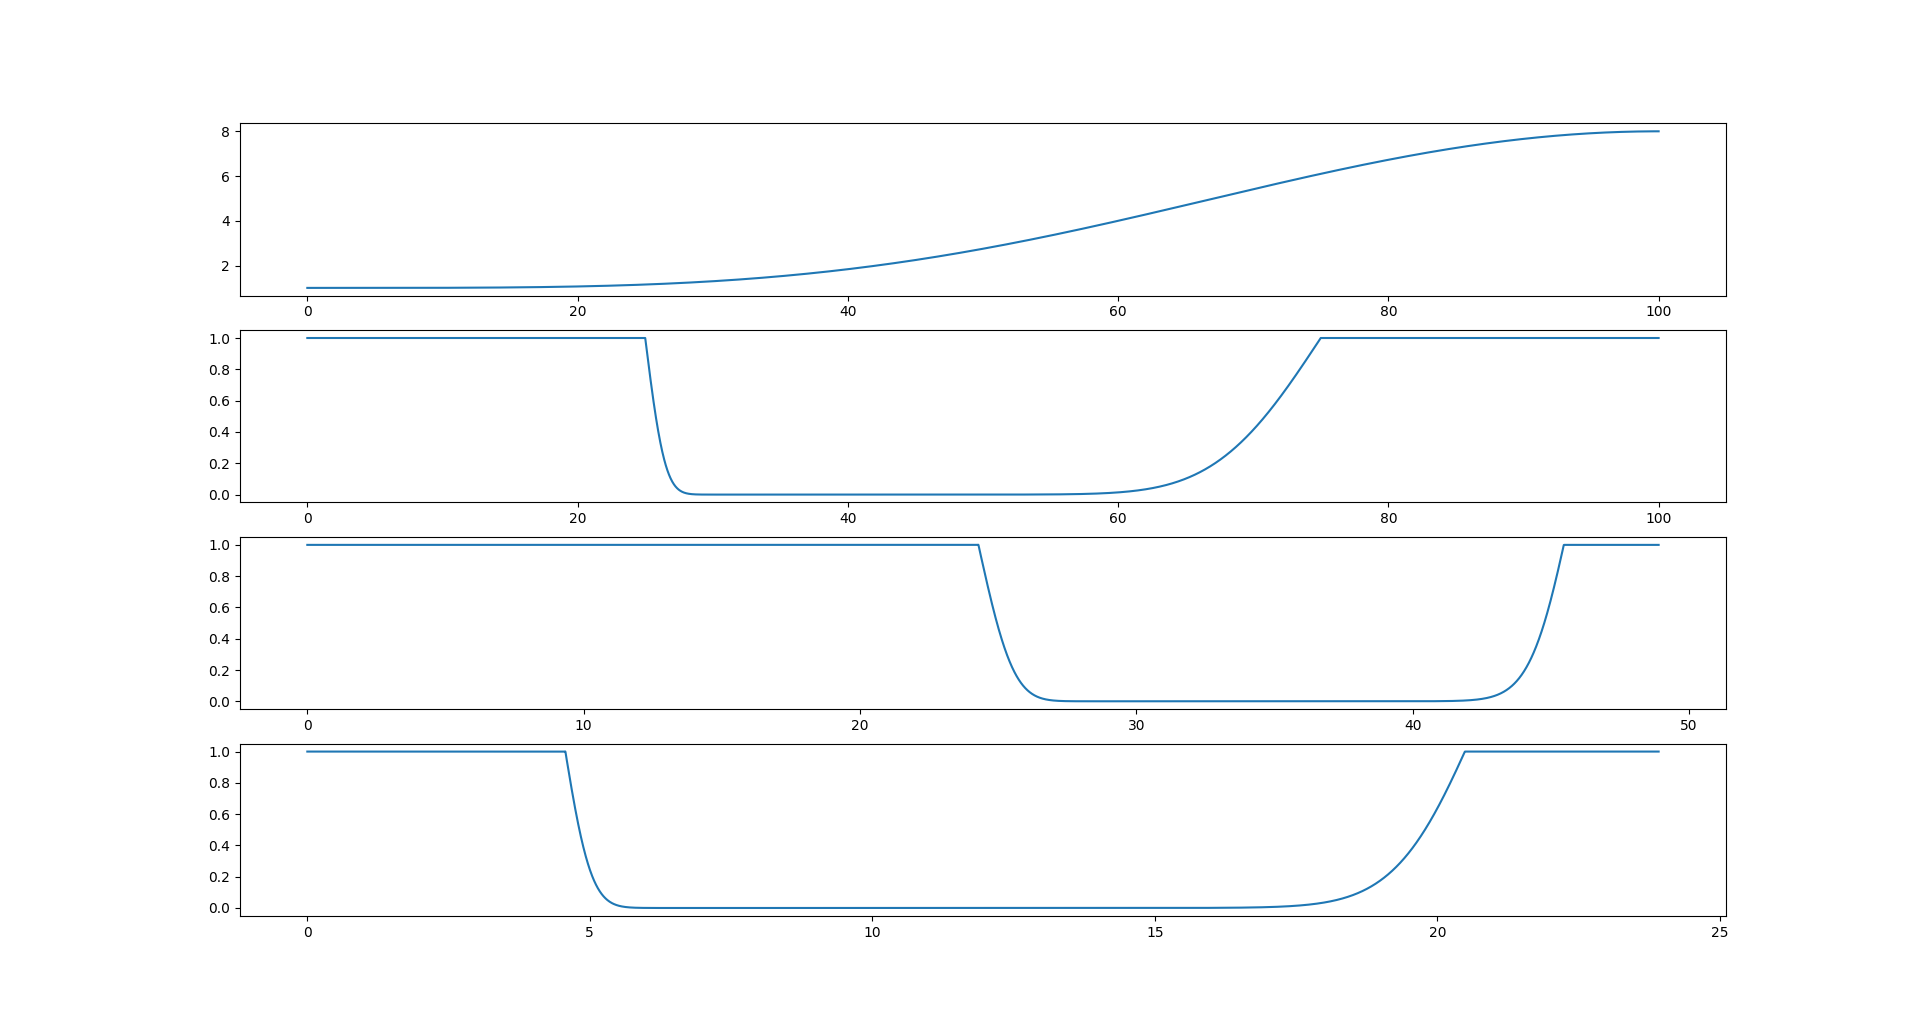
\includegraphics{stretch.png}

\hypertarget{refs}{}
\begin{CSLReferences}{1}{0}
\leavevmode\vadjust pre{\hypertarget{ref-13a}{}}%
{``13.2. {XAFS}: {Pre-edge Subtraction}, {Normalization}, and Data
Treatment --- Xraylarch 0.9.57 Documentation.''} n.d. Accessed December
14, 2021.
\url{https://millenia.cars.aps.anl.gov/xraylarch/xafs_preedge.html\#spectral-deconvolution}.

\leavevmode\vadjust pre{\hypertarget{ref-XRay1991}{}}%
Agarwal, Bipin K. 1991. \emph{X-{Ray Spectroscopy}: An {Introduction}}.
{Berlin, Heidelberg}: {Springer Berlin Heidelberg : Imprint : Springer}.
\url{https://doi.org/10.1007/978-3-540-38668-1}.

\leavevmode\vadjust pre{\hypertarget{ref-Retraction2018}{}}%
Bergmann, Nora, Sébastien Bonhommeau, Kathrin M. Lange, Stefanie M.
Greil, Stefan Eisebitt, Frank de Groot, Majed Chergui, and Emad F. Aziz.
2018. {``Retraction: {On} the Enzymatic Activity of Catalase: An Iron
{L-edge X-ray} Absorption Study of the Active Centre.''} \emph{Physical
Chemistry Chemical Physics} 20 (23): 16294--94.
\url{https://doi.org/10.1039/C8CP91772H}.

\leavevmode\vadjust pre{\hypertarget{ref-Deconvolving2007}{}}%
Fister, T. T., G. T. Seidler, J. J. Rehr, J. J. Kas, W. T. Elam, J. O.
Cross, and K. P. Nagle. 2007. {``Deconvolving {Instrumental} and
{Intrinsic Broadening} in {Excited State X-ray Spectroscopies}.''}
\emph{Physical Review B} 75 (17): 174106.
\url{https://doi.org/10.1103/PhysRevB.75.174106}.

\leavevmode\vadjust pre{\hypertarget{ref-VLSPGM2007a}{}}%
Hu, Y. F., L. Zuin, R. Reininger, and T. K. Sham. 2007. {``{VLS-PGM
Beamline} at the {Canadian Light Source}.''} In \emph{{AIP Conference
Proceedings}}, 879:535--38. {Daegu (Korea)}: {AIP}.
\url{https://doi.org/10.1063/1.2436116}.

\leavevmode\vadjust pre{\hypertarget{ref-Extraction2000}{}}%
Klementiev, Konstantin. 2000. {``Extraction of the {Fine Structure From}
x-Ray {Absorption Spectra}.''} \emph{Journal of Physics D: Applied
Physics} 34 (December): 209.
\url{https://doi.org/10.1088/0022-3727/34/2/309}.

\leavevmode\vadjust pre{\hypertarget{ref-Deconvolution2002}{}}%
Lauer, Tod R. 2002. {``Deconvolution {With} a {Spatially-Variant
PSF}.''} \emph{arXiv:astro-Ph/0208247}, December, 167.
\url{https://doi.org/10.1117/12.461035}.

\leavevmode\vadjust pre{\hypertarget{ref-High2021}{}}%
Nehzati, Susan, Natalia V. Dolgova, Ashley K. James, Julien J. H.
Cotelesage, Dimosthenis Sokaras, Thomas Kroll, Graham N. George, and
Ingrid J. Pickering. 2021. {``High {Energy Resolution Fluorescence
Detected X-ray Absorption Spectroscopy}: {An Analytical Method} for
{Selenium Speciation}.''} \emph{Analytical Chemistry} 93 (26): 9235--43.
\url{https://doi.org/10.1021/acs.analchem.1c01503}.

\leavevmode\vadjust pre{\hypertarget{ref-Larch2013}{}}%
Newville, Matthew. 2013. {``Larch: {An Analysis Package} for {XAFS} and
{Related Spectroscopies}.''} \emph{Journal of Physics: Conference
Series} 430 (April): 012007.
\url{https://doi.org/10.1088/1742-6596/430/1/012007}.

\leavevmode\vadjust pre{\hypertarget{ref-Curve1988}{}}%
Outka, D. A., and J. Stöhr. 1988. {``Curve Fitting Analysis of Near‐edge
Core Excitation Spectra of Free, Adsorbed, and Polymeric Molecules.''}
\emph{The Journal of Chemical Physics} 88 (6): 3539--54.
\url{https://doi.org/10.1063/1.453902}.

\leavevmode\vadjust pre{\hypertarget{ref-Highresolution2007}{}}%
Pratt, Allen, Lucia Zuin, Yun-Mui Yiu, and Sarah Harmer-Bassell. 2007.
{``High-Resolution {XANES S L3},2 Edge Spectra Collected from a Series
of Iron-Bearing Sphalerite({Zn},{Fe}){S} Minerals.''} \emph{Canadian
Journal of Chemistry} 85 (October): 761--66.
\url{https://doi.org/10.1139/v07-072}.

\leavevmode\vadjust pre{\hypertarget{ref-ATHENA2005}{}}%
Ravel, B., and M. Newville. 2005. {``{\emph{ATHENA}} , {\emph{ARTEMIS}}
, {\emph{HEPHAESTUS}} : Data Analysis for {X-ray} Absorption
Spectroscopy Using {\emph{IFEFFIT}}.''} \emph{Journal of Synchrotron
Radiation} 12 (4): 537--41.
\url{https://doi.org/10.1107/S0909049505012719}.

\leavevmode\vadjust pre{\hypertarget{ref-zuin2007early}{}}%
Zuin, Lucia, Yongfeng Hu, and TK Sham. 2007. {``Early Results from the
{VLS-PGM} Beamline at the {Canadian} Light Source {Inc}.''} In
\emph{{JOURNAL OF ELECTRON SPECTROSCOPY AND RELATED PHENOMENA}},
156:XLI--. {ELSEVIER SCIENCE BV PO BOX 211, 1000 AE AMSTERDAM,
NETHERLANDS}.

\end{CSLReferences}

\end{document}
